%%%%%%%%%%%%%%%%%%%%%%%%%%%%%%%%%%%%%%%%%%%%%%%%%%%%%%%%%%%%%%%%%%%%%%%%
%%%%%%%%%%%%%%%%%%%%%% Simple LaTeX CV Template %%%%%%%%%%%%%%%%%%%%%%%%
%%%%%%%%%%%%%%%%%%%%%%%%%%%%%%%%%%%%%%%%%%%%%%%%%%%%%%%%%%%%%%%%%%%%%%%%

%%%%%%%%%%%%%%%%%%%%%%%%%%%%%%%%%%%%%%%%%%%%%%%%%%%%%%%%%%%%%%%%%%%%%%%%
%% NOTE: If you find that it says                                     %%
%%                                                                    %%
%%                           1 of ??                                  %%
%%                                                                    %%
%% at the bottom of your first page, this means that the AUX file     %%
%% was not available when you ran LaTeX on this source. Simply RERUN  %%
%% LaTeX to get the ``??'' replaced with the number of the last page  %%
%% of the document. The AUX file will be generated on the first run   %%
%% of LaTeX and used on the second run to fill in all of the          %%
%% references.                                                        %%
%%%%%%%%%%%%%%%%%%%%%%%%%%%%%%%%%%%%%%%%%%%%%%%%%%%%%%%%%%%%%%%%%%%%%%%%

%%%%%%%%%%%%%%%%%%%%%%%%%%%% Document Setup %%%%%%%%%%%%%%%%%%%%%%%%%%%%

% Don't like 10pt? Try 11pt or 12pt
\documentclass[12pt]{article}
\usepackage[ttdefault=true]{AnonymousPro}
\renewcommand*\familydefault{\ttdefault}
\RequirePackage[T1]{fontenc}

\usepackage{graphicx}

% LaTeX will typeset using Computer Modern Roman, which a lot of
% non-mathematicians and non-engineers won't like. Also, a few PDF
% viewers may not render CMR very well. Instead, Times New Roman can
% be used. That's what this package does.
%\usepackage{times}

% The automated optical recognition software used to digitize resume
% information works best with fonts that do not have serifs. This
% command uses a sans serif font throughout. Uncomment both lines (or at
% least the second) to restore a Roman font (i.e., a font with serifs).
% (NOTE: This requires the times package above)
%\renewcommand{\familydefault}{\sfdefault}

% This is a helpful package that puts math inside length specifications
\usepackage{calc}

% This package helps LaTeX auto-hyphenate hyphenated words if you use
% special hyphens. For example, bio\-/mimicry will properly hyphenate
% ``mimicry'' if necessary.
\usepackage[shortcuts]{extdash}

% Layout: Puts the section titles on left side of page
\reversemarginpar

%
%         PAPER SIZE, PAGE NUMBER, AND DOCUMENT LAYOUT NOTES:
%
% The next \usepackage line changes the layout for CV style section
% headings as marginal notes. It also sets up the paper size as either
% letter or A4. By default, letter was used. If A4 paper is desired,
% comment out the letterpaper lines and uncomment the a4paper lines.
%
% As you can see, the margin widths and section title widths can be
% easily adjusted.
%
% ALSO: Notice that the includefoot option can be commented OUT in order
% to put the PAGE NUMBER *IN* the bottom margin. This will make the
% effective text area larger.
%
% IF YOU WISH TO REMOVE THE ``of LASTPAGE'' next to each page number,
% see the note about the +LP and -LP lines below. Comment out the +LP
% and uncomment the -LP.
%
% IF YOU WISH TO REMOVE PAGE NUMBERS, be sure that the includefoot line
% is uncommented and ALSO uncomment the \pagestyle{empty} a few lines
% below.
%

%% Use these lines for letter-sized paper
\usepackage[paper=letterpaper,
            %includefoot, % Uncomment to put page number above margin
            marginparwidth=1.2in,     % Length of section titles
            marginparsep=.05in,       % Space between titles and text
            margin=0.7in,               % 1 inch margins
            includemp]{geometry}

%% Use these lines for A4-sized paper
%\usepackage[paper=a4paper,
%            %includefoot, % Uncomment to put page number above margin
%            marginparwidth=30.5mm,    % Length of section titles
%            marginparsep=1.5mm,       % Space between titles and text
%            margin=25mm,              % 25mm margins
%            includemp]{geometry}

%% More layout: Get rid of indenting throughout entire document
\setlength{\parindent}{0in}

% Provides special list environments and macros to create new ones
\usepackage[shortlabels]{enumitem}

% Simpler bibsections for CV sections
% (thanks to natbib for inspiration)
%
% * For lists of references with hanging indents and no numbers:
%
%   \begin{bibsection}
%       \item ...
%   \end{bibsection}
%
% * For numbered lists of references (with hanging indents):
%
%   \begin{bibenum}
%       \item ...
%   \end{bibenum}
%
%   Note that bibenum numbers continuously throughout. To reset the
%   counter, use
%
%   \restartlist{bibenum}
%
%   at the place where you want the numbering to reset.

\makeatletter
\newlength{\bibhang}
\setlength{\bibhang}{1em}
\newlength{\bibsep}
 {\@listi \global\bibsep\itemsep \global\advance\bibsep by\parsep}
\newlist{bibsection}{itemize}{3}
\setlist[bibsection]{label=,leftmargin=\bibhang,%
        itemindent=-\bibhang,
        itemsep=\bibsep,parsep=\z@,partopsep=0pt,
        topsep=0pt}
\newlist{bibenum}{enumerate}{3}
\setlist[bibenum]{label=[\arabic*],resume,leftmargin={\bibhang+\widthof{[999]}},%
        itemindent=-\bibhang,
        itemsep=\bibsep,parsep=\z@,partopsep=0pt,
        topsep=0pt}
\let\oldendbibenum\endbibenum
\def\endbibenum{\oldendbibenum\vspace{-.6\baselineskip}}
\let\oldendbibsection\endbibsection
\def\endbibsection{\oldendbibsection\vspace{-.6\baselineskip}}
\makeatother

%% Reference the last page in the page number
%
% NOTE: comment the +LP line and uncomment the -LP line to have page
%       numbers without the ``of ##'' last page reference)
%
% NOTE: uncomment the \pagestyle{empty} line to get rid of all page
%       numbers (make sure includefoot is commented out above)
%
\usepackage{fancyhdr,lastpage}
\pagestyle{fancy}
%\pagestyle{empty}      % Uncomment this to get rid of page numbers
\fancyhf{}\renewcommand{\headrulewidth}{0pt}
\fancyfootoffset{\marginparsep+\marginparwidth}
\newlength{\footpageshift}
\setlength{\footpageshift}
          {0.5\textwidth+0.5\marginparsep+0.5\marginparwidth-2in}
\lfoot{\hspace{\footpageshift}%
       \parbox{4in}{\, \hfill %
                    \arabic{page} of \protect\pageref*{LastPage} % +LP
%                    \arabic{page}                               % -LP
                    \hfill \,}}

% Finally, give us PDF bookmarks
\usepackage{color,hyperref}
\definecolor{darkblue}{rgb}{0.0,0.0,0.3}
\hypersetup{colorlinks,breaklinks,
            linkcolor=darkblue,urlcolor=darkblue,
            anchorcolor=darkblue,citecolor=darkblue}

%%%%%%%%%%%%%%%%%%%%%%%% End Document Setup %%%%%%%%%%%%%%%%%%%%%%%%%%%%


%%%%%%%%%%%%%%%%%%%%%%%%%%% Helper Commands %%%%%%%%%%%%%%%%%%%%%%%%%%%%

%%% HEADING AT TOP OF CURRICULUM VITAE

% The title (name) with a horizontal rule under it
% (optional argument typesets an object right-justified across from name
%  as well)
%
% Usage: \makeheading{name}
%        OR
%        \makeheading[right_object]{name}
%
% Place at top of document. It should be the first thing.
% If ``right_object'' is provided in the square-braced optional
% argument, it will be right justified on the same line as ``name'' at
% the top of the CV. For example:
%
%       \makeheading[\emph{Curriculum vitae}]{Your Name}
%
% will put an emphasized ``Curriculum vitae'' at the top of the document
% as a title. Likewise, a picture could be included:
%
%   \makeheading[{\includegraphics[height=1.5in]{my_picture}}]{Your Name}
%
% the picture will be flush right across from the name. For this example
% to work, make sure the extra set of curly braces is included. Also
% makes ure that \usepackage{graphicx} is somewhere in the preamble.
\newcommand{\makeheading}[2][]%
        {\hspace*{-\marginparsep minus \marginparwidth}%
         \begin{minipage}[t]{\textwidth+\marginparwidth+\marginparsep}%
             {\huge \bfseries #2 \hfill #1}\\[-0.15\baselineskip]%
                 \rule{\columnwidth}{1pt}%
         \end{minipage}}

%%% SECTION HEADINGS

% The section headings. Flush left in small caps down pseudo-margin.
%
% Usage: \section{section name}
\renewcommand{\section}[1]{\pagebreak[3]%
    \vspace{1.3\baselineskip}%
    \phantomsection\addcontentsline{toc}{section}{#1}%
    \noindent\llap{\scshape\smash{\parbox[t]{\marginparwidth}{\hyphenpenalty=10000\raggedright #1}}}%
    \vspace{-\baselineskip}\par}

%%% LISTS

% This macro alters a list by removing some of the space that follows the list
% (is used by lists below)
\newcommand*\fixendlist[1]{%
    \expandafter\let\csname preFixEndListend#1\expandafter\endcsname\csname end#1\endcsname
    \expandafter\def\csname end#1\endcsname{\csname preFixEndListend#1\endcsname\vspace{-0.6\baselineskip}}}

% These macros help ensure that items in outer-type lists do not get
% separated from the next line by a page break
% (they are used by lists below)
\let\originalItem\item
\newcommand*\fixouterlist[1]{%
    \expandafter\let\csname preFixOuterList#1\expandafter\endcsname\csname #1\endcsname
    \expandafter\def\csname #1\endcsname{\let\oldItem\item\def\item{\pagebreak[2]\oldItem}\csname preFixOuterList#1\endcsname}
    \expandafter\let\csname preFixOuterListend#1\expandafter\endcsname\csname end#1\endcsname
    \expandafter\def\csname end#1\endcsname{\let\item\oldItem\csname preFixOuterListend#1\endcsname}}
\newcommand*\fixinnerlist[1]{%
    \expandafter\let\csname preFixInnerList#1\expandafter\endcsname\csname #1\endcsname
    \expandafter\def\csname #1\endcsname{\let\oldItem\item\let\item\originalItem\csname preFixInnerList#1\endcsname}
    \expandafter\let\csname preFixInnerListend#1\expandafter\endcsname\csname end#1\endcsname
    \expandafter\def\csname end#1\endcsname{\csname preFixInnerListend#1\endcsname\let\item\oldItem}}

% An itemize-style list with lots of space between items
%
% Usage:
%   \begin{outerlist}
%       \item ...    % (or \item[] for no bullet)
%   \end{outerlist}
\newlist{outerlist}{itemize}{3}
    \setlist[outerlist]{label=\enskip\textbullet,leftmargin=*}
    \fixendlist{outerlist}
    \fixouterlist{outerlist}

% An environment IDENTICAL to outerlist that has better pre-list spacing
% when used as the first thing in a \section
%
% Usage:
%   \begin{lonelist}
%       \item ...    % (or \item[] for no bullet)
%   \end{lonelist}
\newlist{lonelist}{itemize}{3}
    \setlist[lonelist]{label=\enskip\textbullet,leftmargin=*,partopsep=0pt,topsep=0pt}
    \fixendlist{lonelist}
    \fixouterlist{lonelist}

% An itemize-style list with little space between items
%
% Usage:
%   \begin{innerlist}
%       \item ...    % (or \item[] for no bullet)
%   \end{innerlist}
\newlist{innerlist}{itemize}{3}
    \setlist[innerlist]{label=\enskip\textbullet,leftmargin=*,parsep=0pt,itemsep=0pt,topsep=0pt,partopsep=0pt}
    \fixinnerlist{innerlist}

% An environment IDENTICAL to innerlist that has better pre-list spacing
% when used as the first thing in a \section
%
% Usage:
%   \begin{loneinnerlist}
%       \item ...    % (or \item[] for no bullet)
%   \end{loneinnerlist}
\newlist{loneinnerlist}{itemize}{3}
    \setlist[loneinnerlist]{label=\enskip\textbullet,leftmargin=*,parsep=0pt,itemsep=0pt,topsep=0pt,partopsep=0pt}
    \fixendlist{loneinnerlist}
    \fixinnerlist{loneinnerlist}

%%% EXTRA SPACE

% To add some paragraph space between lines.
% This also tells LaTeX to preferably break a page on one of these gaps
% if there is a needed pagebreak nearby.
\newcommand{\blankline}{\quad\pagebreak[3]}
\newcommand{\halfblankline}{\quad\vspace{-0.5\baselineskip}\pagebreak[3]}

%%% FORMATTING MACROS

% Provides a linked \doi{#1} that links doi:#1 to http://dx.doi.org/#1
\usepackage{doi}
% To change the text before the DOI, adjust this command
%\renewcommand\doitext{doi:}

% Provides a linked \url{#1} that doesn't require escape characters
\usepackage{url}

% You can adjust the style \url{} uses here:
% (options are: same, rm, sf, tt; defaults to tt)
\urlstyle{same}

% For \email{ADDRESS}, links ADDRESS to the url mailto:ADDRESS
% (uncomment to typeset the e\-/mail address in typewriter font;
%  otherwise, will be typeset in the \urlstyle above)
%\DeclareUrlCommand\emaillink{\urlstyle{tt}}
\providecommand*\emaillink[1]{\nolinkurl{#1}}
\providecommand*\email[1]{\href{mailto:#1}{\emaillink{#1}}}

\providecommand\BibTeX{{B\kern-.05em{\sc i\kern-.025em b}\kern-.08em \TeX}}
\providecommand\Matlab{\textsc{Matlab}}

% Custom hyphenation rules for words that LaTeX has trouble with
\hyphenation{bio-mim-ic-ry bio-in-spi-ra-tion re-us-a-ble pro-vid-er Media-Wiki}

%%%%%%%%%%%%%%%%%%%%%%%% End Helper Commands %%%%%%%%%%%%%%%%%%%%%%%%%%%

%%%%%%%%%%%%%%%%%%%%%%%%% Begin CV Document %%%%%%%%%%%%%%%%%%%%%%%%%%%%

\begin{document}
\makeheading{Guilherme Oliveira}

\section{Contact Information}

% NOTE: Mind where the & separators and \\ breaks are in the following
%       table. Table is one row made up of three parboxes. The left
%       parbox has address info, the middle parbox has a vertical bar,
%       and the right parbox has phone and electronic contact
%       information.
%
% MACROS: \rcollength is the width of the right column of the table
%             (adjust it to your liking; default is 1.85in).
%         \spacewidth is width of area between left and right boxes.
%
\newlength{\rcollength}\setlength{\rcollength}{1.85in}%
\newlength{\spacewidth}\setlength{\spacewidth}{20pt}
%
\begin{tabular}[t]{@{}p{\textwidth-\rcollength-\spacewidth}@{}p{\spacewidth}@{}p{\rcollength}}%

% Address box
\parbox{\textwidth-\rcollength-\spacewidth}{%
\begin{tabular}{ll}
Address: & Wisbyer Strasse 63, Berlin \\
Mobile: & +49 6570 8332 \\
Skype: & guilherme\_flex \\
E-mail: & \email{ghophp@gmail.com} \\
Born: & 29 September 1991 \\
Nationality: & Brazilian \\
Portfolio: & \href{http://ghophp.github.io}{ghophp.github.io}
\end{tabular}}

&
% Uncomment to add a vertical bar in middle of contact information
%{\vrule width 0.5pt}
\parbox[m][5\baselineskip]{\spacewidth}{} &

% Non-snail-mail contact information
\parbox{\rcollength}{%
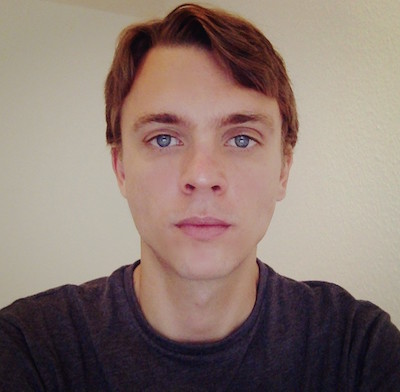
\includegraphics[width=.25\textwidth]{photo}}
\end{tabular}

%%
%% In modern CV's, it seems like ``Objective'' is frowned upon. Instead,
%% incorporate it into a well-constructed cover letter. The ``More
%% information'' can go at the end of the CV, but it should not distract
%% from the section giving references available to contact.
%%
%
% \section{Objective}
%
% Placement in an academic position (i.e., faculty, postdoctoral, or
% research scientist) that allows for advanced research in distributed
% complex adaptive systems (i.e., modeling, analysis, design, and
% verification) with a particular focus on the control of engineered
% agents (e.g., for communications, control, software, electronics, and
% sustainability) and the analysis of biological phenomena (e.g.,
% self-organization, ecological rationality)
% \begin{innerlist}
% \item More information and auxiliary documents can be found at\\\url{http://www.tedpavlic.com/facjobsearch/}
% \end{innerlist}

\section{Keywords}

\textbf{problem solver, fast learner, agile integrant, language agnostic, database normaliser, rest advocate}

\section{Core Competencies}

\begin{innerlist}
	\item Rapid understanding of new code bases and new technologies in general.
	\item Requirements analysis and breakdown, software architecture and design.
	\item Capability to code for multiple platforms in multiple programming languages.
	\item A loyal team member devoted to achieve the goals together.
	\item Curious and adaptive learner always seeking new challenges.
\end{innerlist}

\section{Results Accomplished}

\begin{innerlist}
	\item Co-founder of a business providing optical character recognition services for \href{https://en.wikipedia.org/wiki/APM_Terminals}{APM Terminals}.
	\item Helped big corporations (such as \href{https://pt.wikipedia.org/wiki/Grupo_Votorantim}{Votorantim Group}) to connect with their customers through the development and release of iOS and Android applications.
	\item Contributed to open-source project and pushed inside private companies for a more active and professional open-source presence.
	\item Directly involved in successfully implementing CI/CD processes with micro-services architecture.
	\item Top grades and final paper award which guaranteed immediate enrollment in master's degree at highly disputed federal institution.
\end{innerlist}

\section{Awards}

\begin{innerlist}
	\item Best Final Paper of University 2013 (Software Prototype to Auxiliate and Stimulate the Corporal Stretching Process) - \href{https://github.com/ghophp/kinect-body-position}{Github Source}
\end{innerlist}

\section{Professional Experience}

\textbf{Onefootball GmbH},
Berlin, Germany
\begin{outerlist}

    \item[] \textit{Senior Backend Engineer}%
            \hfill \textbf{August 2015 to present}\\
			I am directly involved on the implementation of CI/CD systems to improve the deployment and scalability process. We use parts of Agile methodology to coordinate the processes. New services inside the micro-service architecture are being created with Golang and we still maintain services written in PHP.
			
\end{outerlist}

\halfblankline

\textbf{yetu AG},
Berlin, Germany
\begin{outerlist}

    \item[] \textit{Senior Software Engineer}%
            \hfill \textbf{2015}\\
			At yetu I was working with Scala, Play Framework and Akka. The systems were distributed into a complex automated structure managed by Ansible and covered by different types of tests (unit, functional, integration, end-to-end). We used Agile as our base methodology with aspects from Kanban and Scrum.

\end{outerlist}

\halfblankline

\textbf{Five Intl Systems},
Itajai, Brazil
\begin{outerlist}

    \item[] \textit{Cofounder \& CTO}%
            \hfill \textbf{February 2014 to April 2015}\\
			Me and three other associates created a company focused on port solutions, specifically a solution for optical character recognition. The system was written in C++ with Qt and was installed into a few entry gates for the Itajai Port in Brazil. APM Terminals was the first customer with venue estimated in \$4.24 billions.
			
\end{outerlist}

\halfblankline

\textbf{Coderockr AG},
Joinville, Brazil
\begin{outerlist}

    \item[] \textit{Senior Software Engineer}%
            \hfill \textbf{March 2014 to April 2015}\\
			Full Stack developer working with systems for the web in a very productive methodology that aggregates some parts of Scrum and Kanban. Also worked with Android apps releasing large distributed systems such as a social network named SocialBase.
			
\end{outerlist}

\halfblankline

\textbf{Freelancer},
Brazil
\begin{outerlist}

    \item[] \textit{Senior Software Engineer}%
            \hfill \textbf{March 2009 to 2015}\\
			In order to fulfill my passion for innovative projects and increase my networking, I have worked as a freelancer for many clients. From international projects to manage more than 5 million hectares of forest in Canada, to mobile application to track orders in restaurants. I always cherish the delivery and quality, with a service that does not tie the client, trying to deliver what was asked, leaving the option of the contract extension as a choice based on the quality of my work.
			
\end{outerlist}

\halfblankline

\textbf{Humantech - Knowledge Management},
Joinville, Brazil
\begin{outerlist}

    \item[] \textit{Head of Development}%
            \hfill \textbf{March 2009 to March 2014}\\
			I started to work at Humantech at the age of 17 as an intern at the same time as the university course. After 6 months I was admitted as a junior software developer, few years later I had my own team to manage. The chaotic outsourcing environment helped me to discover that I am passionate for research and development.
			
\end{outerlist}

\section{Education}

\textbf{Mastering in Applied Computer Science}
\begin{outerlist}

    \item[] \textit{UDESC}%
            \hfill \textbf{2014 - Unfinished}\\
            After finishing bachelor I enrolled to master's degree in one of the best universities of the country in matters of technology. After a semester with some good disciplines that improved my research skills, my line of research and the focus on academy didn't interest me. With the offer to move to Berlin, I left the master's unfinished.
			
\end{outerlist}

\halfblankline

\textbf{Bachelor's in Information Technology}
\begin{outerlist}

    \item[] \textit{UNISOCIESC}%
            \hfill \textbf{2009 - 2013}\\
            In college I was one of the top students because I have been working since the beginning. I won the prize Best Final Paper of University 2013 which later helped me to be accepted at the master's.
			
\end{outerlist}

\halfblankline

\textbf{Technician Informatics}
\begin{outerlist}

    \item[] \textit{SENAI}%
            \hfill \textbf{2006 - 2008}\\
            At the age of 15 I started to study at technician level, along with high school. This course was a life changer, it has given me during early ages a meaning in life. When I started to understand how to program a computer, I knew that this is what I wanted to do for living.
			
\end{outerlist}

\section{Programming skills}

\textbf{strong} Golang, PHP, SQL, JavaScript, HTML, CSS \& Java
%

\halfblankline

\textbf{moderate} Python, Scala, C++, ActionScript 3 \& Regular Expressions
%

\halfblankline

\textbf{have used} Objective-C,Shell scripting, C\#, AutoLISP \& LaTeX
%

\section{Concepts \break Knowledge}

rest, database normalisation, \href{https://guides.github.com/introduction/flow/}{github flow}, git flow, micro-services \& monolith architecture, continuous integration \& deployment, refactoring strategies, system design, agile \& kanban methodologies, message systems, protocols

\section{Frameworks \& Tools}

\textbf{strong} git, Sublime Text, Terminal, RabbitMQ, Redis, Memcached, MySQL, Travis, AngularJS, GruntJS, Bower, Martini, Android SDK, Zend, Symphony \& Doctrine
%

\halfblankline

\textbf{moderate} BuildBot, MongoDB, EC2, RDS, OpsWorks, Play Framework, NodeJS, Python Twisted \& Cyclone, Socket.io, DNS, Unix, Firewall \& Qt
%

\halfblankline

\textbf{have used} Hibernate, Akka, ReactJS, BackboneJS, Realm.io, XCode \& Elastic Beanstalk
%

\section{Natural Languages}

Portuguese (mother tongue), English (fluent), Spanish (moderate) \& German (beginner).

\section{Coworkers References}

\href
{https://de.linkedin.com/in/larsalexanderblumberg/en}
{\textbf{Lars Alexander Blumberg}} (Head of Software Engineering) \break
%
Guilherme is not only a very careful and fast learning software engineer, but is also able to adopt very quickly to new software components, languages and patterns. He was also an outstanding team colleague, his sharp mind, gentleness and willing to always improve make Guilherme a very valuable team member. I would be very proud if I had the chance to work with him again.

\halfblankline

\href
{https://www.linkedin.com/in/jonecir}
{\textbf{Jonecir Souza}} (Experienced Senior IT Professional) \break
%
For the past five years, I have been working with Guilherme. Since then, I have gotten to know him quite well and can thoroughly vouch for his character, professionalism and technical abilities. I have worked with him on close to 15 different IT projects, and I have been constantly impressed with both his technical skills and performance in our field.

\halfblankline

\href
{https://nl.linkedin.com/in/espeiorin}
{\textbf{Andre Espeiorin}} (iOS Developer) \break
%
Guilherme is a talented language-agnostic programmer. No matter which language, he always begins with the problem itself, this is a rare characteristic nowadays. Also he has a great team spirit and this makes him easy to fit in any high skilled team.

% The ``More Info'' section may not be necessary; make sure it's short
% so it doesn't prevent people from seeing references available to
% contact.
\section{More Information}

More information can be found at\\%
\url{http://ghophp.github.io/}.

\end{document}

%%%%%%%%%%%%%%%%%%%%%%%%%% End CV Document %%%%%%%%%%%%%%%%%%%%%%%%%%%%%

%----------------------------------------------------------------------%
% The following is copyright and licensing information for
% redistribution of this LaTeX source code; it also includes a liability
% statement. If this source code is not being redistributed to others,
% it may be omitted. It has no effect on the function of the above code.
%----------------------------------------------------------------------%
% Copyright (c) 2007, 2008, 2009, 2010, 2011 by Theodore P. Pavlic
%
% Unless otherwise expressly stated, this work is licensed under the
% Creative Commons Attribution-Noncommercial 3.0 United States License. To
% view a copy of this license, visit
% http://creativecommons.org/licenses/by-nc/3.0/us/ or send a letter to
% Creative Commons, 171 Second Street, Suite 300, San Francisco,
% California, 94105, USA.
%
% THE SOFTWARE IS PROVIDED "AS IS", WITHOUT WARRANTY OF ANY KIND, EXPRESS
% OR IMPLIED, INCLUDING BUT NOT LIMITED TO THE WARRANTIES OF
% MERCHANTABILITY, FITNESS FOR A PARTICULAR PURPOSE AND NONINFRINGEMENT.
% IN NO EVENT SHALL THE AUTHORS OR COPYRIGHT HOLDERS BE LIABLE FOR ANY
% CLAIM, DAMAGES OR OTHER LIABILITY, WHETHER IN AN ACTION OF CONTRACT,
% TORT OR OTHERWISE, ARISING FROM, OUT OF OR IN CONNECTION WITH THE
% SOFTWARE OR THE USE OR OTHER DEALINGS IN THE SOFTWARE.
%----------------------------------------------------------------------%
